\chapter{Εισαγωγή}

\section{Ενισχυτική Μάθηση}
Η ενισχυτική μάθηση (ΕΜ) (\en{Reinforcement Learning (RL)}) είναι είναι ένας γενικός όρος που έχει
δοθεί σε μια οικογένεια τεχνικών στις οποίες το σύστημα προσπαθεί να μάθει μέσα από την άμεση αλληλεπίδραση
με το περιβάλλον.\cite{aigreek} Είναι τομέας της τεχνητής νοημοσύνης και, πιο συγκεκριμένα, της μηχανικής μάθησης.

Πιο συγκεκριμένα, η ΕΜ είναι η διαδικασία κατα την οποία ένας πράκτορας (\en{agent}) αλληλεπιδρά με το περιβάλλον του,
και μαθαίνει τι να κάνει, παρατηρώντας τις συνέπειες των ενεργειών του (\en{actions}).
Ο πράκτορας δεν δίνεται πληροφορίες σχετικά με το ποίες ενέργειες να επιλέξει, αλλά πρέπει να
ανακαλύψει ποιες δράσεις προσφέρουν την μέγιστη ανταμοιβή (\en{reward}), δοκιμάζοντας τες \cite{rlbook}.
Επιπλέον, σε πολλές περιπτώσεις οι ενέργειες του πράκτορα δεν επηρεάζουν μόνο την άμεση ανταμοιβή,
αλλά και από την ανταμοιβή στην επόμενη κατάσταση και πιθανώς και όλες τις επόμενες ανταμοιβές.
Σύμφωνα με τα παραπάνω, η ΕΜ στοχεύει να λύσει προβλήματα μέσω τεχνικών
\textit{δοκιμής-και-λάθους \en{(trial-and-error)}} σε περιβάλλοντα με \textit{καθυστερημένες ανταμοιβές}.

Η θεωρία της ΕΜ βασίζεται πάνω στην υπόθεση της ανταμοιβής (\en{reward hypothesis}), στην ιδέα ότι κάθε στόχος μπορεί να
εκφραστεί ως η μεγιστοποίηση την αναμενόμενης αξίας του σωρευτικού (\en{cummulative}) αθροίσματος ενός μονοδιάστατου σήματος
(ανταμοιβής). Με απλά λόγια, η υπόθεση θέτει την ιδέα ότι κάθε στόχος μπορεί να εκφραστεί σαν την μεγιστοποίηση μιας ανταμοιβής.
Η ανταμοιβή αυτή δεν χρειάζεται να είναι θετικός αριθμός, μπορεί να είναι και αρνητικός. Για παράδειγμα, αν ο στόχος είναι η
'εξοδος από ένα λαβύρινθο, η ανταμοιβή μπορεί να είναι αρνητική σε κάθε βήμα μέχρι την έξοδο, ώστε τελικά η στόχος να είναι η
ελαχιστοποίηση της απόλυτης τιμής της ανταμοιβής.

Το πεδίο της ΕΜ έχει τις ρίζες του σε δύο περιοχές. Η πρώτη είναι η συμπεριφορική ψυχολογία, από όπου προέρχεται το
παράδειγμα της δοκιμής-και-λάθους, και η δεύτερη είναι η περιοχή του βέλτιστου ελέγχου, από όπου η ΕΜ δανείζεται
τον μαθηματικό φορμαλισμό (κυρίως τον δυναμικό προγραμματισμό) που υποστηρίζει το πεδίο. H ΕΜ
βρίσκονται στην τομή πολλών διαφορετικών επιστημονικών πεδίων, οι οποίοι φαίνται στο Σχήμα~\ref{fig:faces_rl}\cite{silver2015}.

\begin{figure}[h]
    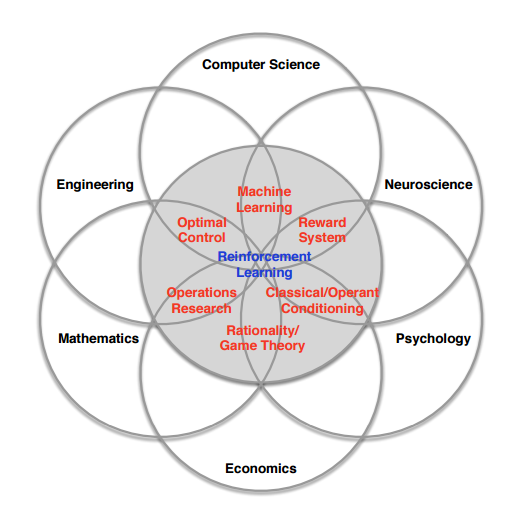
\includegraphics[width=0.5\textwidth]{body_matter/chapter1/images/faces_of_rl.png}
    \Centering
    \caption{Τα πρόσωπα της ενισχυτικής μάθησης}
    \label{fig:faces_rl}
\end{figure}

Η ΕΜ πολλές φορές συγχέεται με τις άλλες τεχνικές μηχανικής μάθησης, παρόλο που έχει αρκετά σημαντικές διαφορές.
Αρχικά, η κύρια διαφορά μεταξύ της επιτηρούμενης μάθησης (\en{supervised learning}) και της ΕΜ είναι ότι στην επιτηρούμενη
μάθηση, το μοντέλο εκπαιδεύεται πάνω σε δείγματα (\en{samples}) και ετικέτες (\en{labels}), και κάθε πρόβλεψη θεωρείται
μοναδικό γεγονός. Από την άλλη, στην ΕΜ, μπορούν να υπάρχουν πολλά βήματα πριν ο πράκτορας μάθει αν η απόφαση που πήρε ήταν
σωστή, και μπορεί να μην μάθει ποτέ ποια ήταν η αληθής/βέλτιστη τιμή, αλλά να βλέπει μόνο την επίδραση που είχαν οι πράξεις
του στο περιβάλλον.


\subsection{Γενικά}

Πιο φορμαλιστικά, σε ένα περιβάλλον ΕΜ, ένας αυτόνομος πράκτορας, ελεγχόμενος από ένα αλγόριθμο μηχανικής μάθησης,
παρατηρεί μια κατάσταση $s_t$ από το περιβάλλον του σε ένα χρονικό βήμα $t$. Οι καταστάσεις προέρχονται από τον
χώρο καταστάσεων $\mathcal{S}$. Ο πράκτορας αλληλεπιδρά με το περιβάλλον επιλέγοντας μια δράση $a_t$ με βάση την κατάσταση
$s_t$, επιλεγμένη από ένα χώρο δράσεων $\mathcal{A}$. Όταν ο πράκτορας επιλέξει την δράση, τότε τόσο το περιβάλλον,
οσο και ο πράκτορας μεταβαίνουν σε μια νέα κατάσταση $s_{t+1}$, με βάση την τρέχουσα κατάσταση και την επιλεγμένη
δράση \cite{drlbs}.

Ο πράκτορας επίσης λαμβάνει και μια μονοδιάστατη ανταμοιβή $R_t$ η οποία προέρχεται από το ζεύγος κατάστασης-δράσης. Αυτή η
ανταμοιβή δρα ως μια μορφή ανατροφοδότησης για τις δράσεις του πράκτορα. Επιπλέον, ο πράκτορας διατηρεί μια αντιστοίχηση μεταξύ
κατάστασης και δράσης, η οποία συμβολίζεται ως $π(a_t | s_t)$. Για κάθε ζευγάρι κατάστασης-δράσης, υπάρχει η αντίστοιχη ανταμοιβή $R$
που λαμβάνει ο πράκτορας ως αποτέλεσμα μια συγκεκριμένης δράσης $a_t$ στην κατάσταση $s_t$. Η βέλτιστη σειρά δράσεων προσδιορίζεται
από αυτές τις ανταμοιβές που προμηθεύει το περιβάλλον. Ο τελικός στόχος του πράκτορα είναι να μάθει μια πολιτική $π$, η οποία μεγιστοποιεί
την αναμενόμενη απόδοση (σωρευτική, εκπτωθείσα (\en{discounted}) ανταμοιβή). Δοθείσας μιας κατάστασης η πολιτική επιστρέφει την επόμενη δράση την οποία θα κάνει ο πράκτορας.
Μια βέλτιστη πολιτική είναι η πολιτική η οποία μεγιστοποιεί την αναμενόμενη απόδοση στο συγκεκριμένο περιβάλλον.

Θέλουμε τα προβλήματα ΕΜ που ασχολούμαστε να ικανοποιούν την Μαρκοβιανή ιδιότητα. Δηλαδή, για κάθε κατάσταση, το μέλλον να εξαρτάται μόνο από
την τρέχουσα κατάσταση και όχι τις προηγούμενες. Όταν ισχύει αυτή η ιδιότητα τότε μπορούμε να μοντελοποιήσουμε το πρόβλημα ως μια Μαρκοβιανή
Διαδικασία Αποφάσεων (\en{Markov Decision Process}), η οποία αποτελείται από:
\begin{itemize}
    \item ένα σύνολο από καταστάσεις $\mathcal{S}$, και επιπλέον μια κατανομή αρχικών καταστάσεων $p(s_0)$,
    \item ενα σύνολο από δράσεις $\mathcal{A}$,
    \item τις πιθανότητες μετάβασης μεταξύ των καταστάσεων \\ $\Pr{\{S_t=s'|S_{t-1}=s, A_{t-1}=a\}}$, οι οποίες αντιστοιχούν ένα ζεύγος
          κατάστασης-δράσης την στιγμή $t-1$ σε μια κατανομή καταστάσεων την στιγμή $t$,
    \item μια συνάρτηση άμεσης ανταμοιβής $R(s_{t-1}, a_{t-1}, s_t)$,
    \item κατα τον υπολογισμό της σωρευτικής ανταμοιβής, συμπεριλαμβάνεται και ένας παράγοντας "έκπτωσης" $\gamma \in [0,1]$, ο οποίος
          χρησιμοποιειται για να τοποθετηθεί μικρότερη έμφαση στις πιο παλιές ανταμοιβές.
\end{itemize}

Σύμφωνα με τα παραπάνω, ορίζουμε ως την απόδοση την εκπτωθείσα, σωρευτική ανταμοιβή μαζί με τον παράγοντα έκπτωσης:
\begin{equation}
    R_t = \sum_{k=0}^{\infty}{\gamma^k r_{t+k}}
\end{equation}

Ένα κύριο χαρακτηριστικό κάθε μεθόδου ΕΜ είναι η \textbf{συνάρτηση αξίας}, μια πρόβλεψη της αναμενόμενης, σωρευτικής, εκπτωθείσας, μέλλουσας
απόδοσης. Ποσοτικοποιεί πόσο καλή είναι μια κατάσταση ή ένα ζεύγος κατάστασης-δράσης. Η αξία μιας κατάστασης
\begin{equation}
    \upsilon_\pi(s) =\mathbb{E}[R_t | s_t = s]
\end{equation}

είναι η αναμενόμενη απόδοση ακολουθώντας την πολιτική $π$ από την κατάσταση $s$. Η αξία της δράσης
\begin{equation}
    q_\pi(s,a) =\mathbb{E}[R_t | s_t = s, a_t = a]
\end{equation}
είναι η αναμενόμενη απόδοση της επιλογής της δράσης $a$ στην κατάσταση $s$ και ακολουθώντας την πολιτική $π$ μετά.

Επιπλέον, για να περιγράψουμε καλύτερα τις μεθόδους ΕΜ, τις χωρίζουμε σε μεθόδους που λύνουν προβλήματα
\textbf{βασισμένα σε μοντέλο \en{(model-based)}} ή προβλήματα \textbf{ανεξάρτητα μοντέλου \en{(model-free)}}.

Moreover, to better describe RL methods we divide them in
\textbf{model-based} and \textbf{model-free} problems. \textbf{Model-based} methods are used when we have a
complete knowledge of the dynamics of the surrounding environment and rely on \textit{planning} as their primary component.
The methods include dynamic programming and similar methods. We use policy evaluation to calculate the return of a specific policy and
On the other hand \textbf{model-free} methods require no prior knowledge of the environment and rely on \textit{learning}.
By a \textit{model} of the environment we mean anything that an agent can use to predict how the environment will respond to
its actions.

